\documentclass[a4paper,10pt]{article}
\usepackage[english]{babel}
\usepackage[utf8]{inputenc}
\usepackage{url}
\usepackage[margin=1in]{geometry}
\usepackage{enumitem}

\usepackage[nottoc]{tocbibind}
\usepackage{fancyvrb} 
\usepackage{float}
\usepackage{graphicx}
\usepackage{subcaption}
\usepackage{color}
\usepackage{booktabs}
\usepackage{listings}

\title{Combinatorial Optimization\\Homework 3 – Experimental Measurements}
\author{Matyáš Skalický\\skalimat@fit.cvut.cz}

\begin{document}
\maketitle
\tableofcontents
\medskip


\section{Measured Algorithms}

Baseline exact method is the \textbf{brute-force} algorithm that recursively iterates explores all possible solutions without any speedups or pruning.

The \textbf{branch\&bound} extends the brute-force with 2 speedups. We stop when the current candidate already exceeds the capacity of a bag. Also, we don't recurse further when the cost sum of the items that can be added into the bag is lower than the best found solution.

The dynamic programming approach is based on the \textbf{decomposition by cost}. This solution is based on memoization by the recursive function calls by returning the maximum value from the tested branches on return.

The \textbf{greedy} heuristic simply adds the items with the highest cost/weight ratio until the capacity of the bag is reached. This is the only algorithm that doesn't always result in the optimal solution.

\section{Measured Variables}
For the pilot experiments, I've chosen to benchmark all algorithms on the instances of size $24$. The generator's maximum weight $W$ is set to $3000$ as well as maximum price $C$.

In the following experiments, we will try to measure how time and the solution quality depend on the generator inputs. Also, we will look how robust each algorithm is against permutations in the algorithm inputs.

\begin{itemize}
	\item Ratio of bag capacity to summary weight. (\lstinline{cw_ratio} $\in [0, 1]$)
	\item Correlation between price and weight. (\lstinline{pw_corr} $\in \{\textit{uni}, \textit{corr}, \textit{strong}\}$)
	\item Granularity and distribution of weights. (\lstinline{w_dist} $\in \{\textit{light}, \textit{bal}, \textit{heavy}\}$)
\end{itemize}

\clearpage

\section{Experiments}
We will measure the effect of each variable separately. We will generate 10 problem instances for each algorithm with each weight.

\subsection{Robustness}
First, we will try to answer the robustness (invariance to order of input items) of each algorithm. We will use default generator values mentioned above. We will generate 500 instances and calculate 10 permutations for each algorithm. We will calculate the variance in the elapsed time across the 10 permutations and take a mean across all generated instances.

\begin{table}[!htb]
\centering
\begin{tabular}{lrr}
method & mean runtime & mean runtime variance\\
\midrule
greedy heuristic & 0.00006964 & 0.00000001 \\
branch\&bound & 0.00642724 & 0.00001817 \\
dynamic (cost) & 0.38064328 & 0.01843123 \\
bruteforce   & 9.22061772 & 1.95676123 \\
\bottomrule
\end{tabular}
\caption{Mean of runtime (seconds) and runtime variance over 10 permutations}
\end{table}

It is not surprising, that the heuristic is extremely stable as it is basically just one pass over the items in the bag. I have expected that the algorithms such as branch\&bound and dynamic would be less robust as especially the first one depends on the order of items while pruning. Yet the dynamic algorithm seems unstable (not robust to the item premutations) as well.

It is surprising that the bruteforce algorithm shows such huge mean variance in the measured runtime. But it is also worth noting that the mean runtime for bruteforce was $9.22$ seconds while it was only $0.38$ and $0.006$ seconds for dynamic and branch\&bound respectively.

I would say, that since the measured metric was the runtime and the experiments were performed on a 40-core CPU in parallel, it could be caused by uneven load across CPU cores as different tasks were running on the CPU as well. But I still find it very interesting.

\subsection{Pilot Experiments}

 We will not measure the permutations in the pilot experiments. Figure \ref{pilot_figure} contains the absolute Pearson correlation between the runtime in seconds and changing parameters in the instance generator.

\begin{figure}[!htb]
	\centering
  	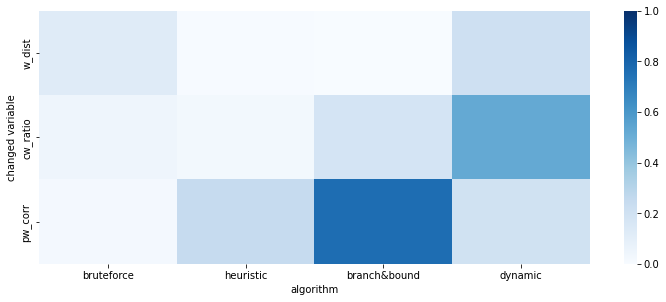
\includegraphics[width=\textwidth]{images/pilot.png}
	\caption{Correlation (absolute) of the algorithm runtime to the change in parameters}
	\label{pilot_figure}
\end{figure}

\subsection{Detailed Experiments}

Based on the Figure \ref{pilot_figure}, we can see that there is a strong correlation between \emph{dynamic} and \lstinline{cw_ratio}. We will further inspect the relation of \emph{dynamic} and \lstinline{w_dist}. For the \emph{branch\&bound}, we will inspect the variables \lstinline{cw_ratio} and \lstinline{pw_corr} as they has shown a small correlation with the algorithm runtime.

All variables were tested separately, 100 samples per each testing instance size.

\subsubsection{Weight Distribution (w\_dist)}

\begin{figure}[!htb]
	\centering
  	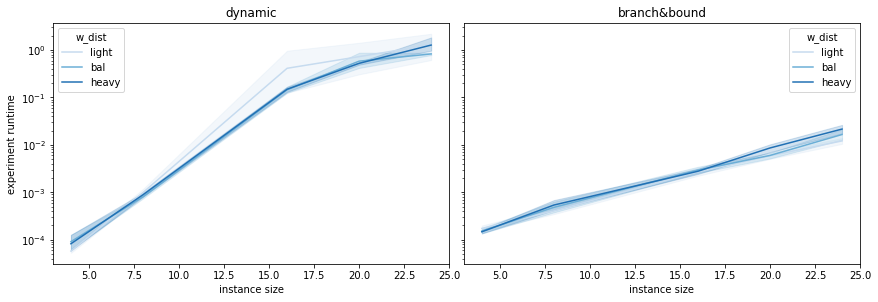
\includegraphics[width=\textwidth]{images/wdist.png}
	\caption{Weight distribution [light, bal, heavy]}
	\label{wdist}
\end{figure}

Weight distribution affects whether the majority of the items are light, heavy, or balanced. As indicated by the pilot experiments, the weight distribution (as seen in Figure \ref{wdist}) does not heavily the experiment runtime.

\subsubsection{Price and Weight Correlation (pw\_corr)}

\begin{figure}[!htb]
	\centering
  	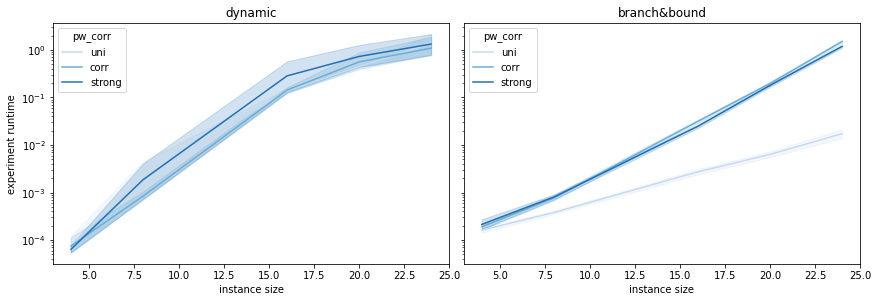
\includegraphics[width=\textwidth]{images/pwcorr.png}
	\caption{Price and Weight Correlation [uni, corr, strong]}
	\label{pwcorr}
\end{figure}

As shown in the Figure \ref{pwcorr}, dynamic programming isn't affected by the changing correlation between price and weight (\lstinline{pw_corr}). On the other hand, we can see that branch\&bound is affected strongly as the processing speed of the bags with correlated items is much slower. This is likely due to the pruning being less effective. 

\clearpage

\subsubsection{Capacity and Weight Ratio (cw\_ratio)}

The \lstinline{cw_ratio} is defined as the ratio of max knapsack capacity to total weight. The pilot experiments had indicated a correlation between the runtime and this variable. Figure \ref{cwratio} sheds more light to this hypothesis. Both dynamic and branch\&bound algorithms are affected by the changing \lstinline{cw_ratio}.

\begin{figure}[!htb]
	\centering
  	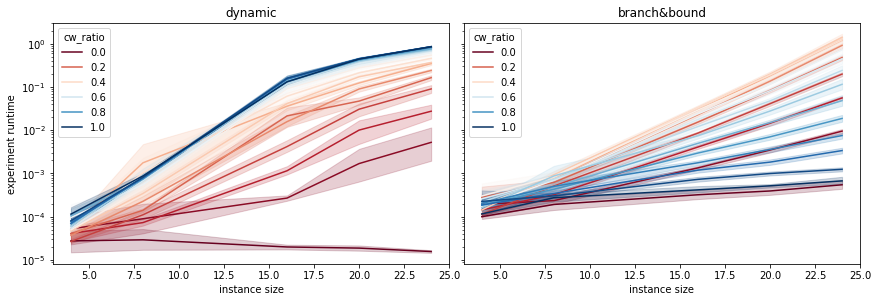
\includegraphics[width=\textwidth]{images/cwratio.png}
	\caption{Ratio of max knapsack capacity to total weight}
	\label{cwratio}
\end{figure}

As seen from the Figure \ref{cwratio_relation}, the dynamic algorithm is strongly affected if \lstinline{cw_ratio} is closer to $1$. The relationship for the brach\&bound isn't linear. The algorithm is the fastest both, for bags which were on the sides of the spectrum.

\begin{figure}[!htb]
	\centering
  	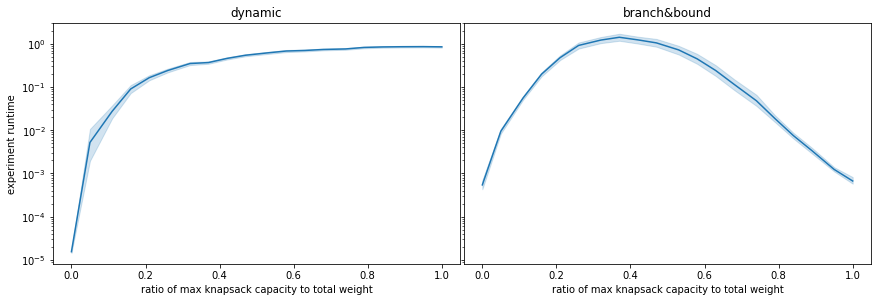
\includegraphics[width=\textwidth]{images/cwratio_fixed.png}
	\caption{ratio of max knapsack capacity to total weight for instance size 24}
	\label{cwratio_relation}
\end{figure}


\section{Discussion and Takeoffs}

I've first ran the pilot experiments on the small data samples to detect potentially interesting relationships between generator hyperparameters and the experiment runtime. Based on this, I've explored the effects of the parameters on larger data samples as mentioned above to see the relationships in a better detail.

One of the interesting takeoffs for me was the large variance in the brute-force algorithm when permuting the items. As the brute-force algorithm always searches through the full searchspace, the time taken should be very similar. My intuition about this is that this must be due to uneven CPU thread scheduling.

Overall, I would say that this homework took a long time to create, yet I wish I was doing anything useful. Instead of just replicating the experiments that were done 1000 times before and don't benefit anyone in doing again in our homeworks.


\end{document}